\begin{figure}
\centering
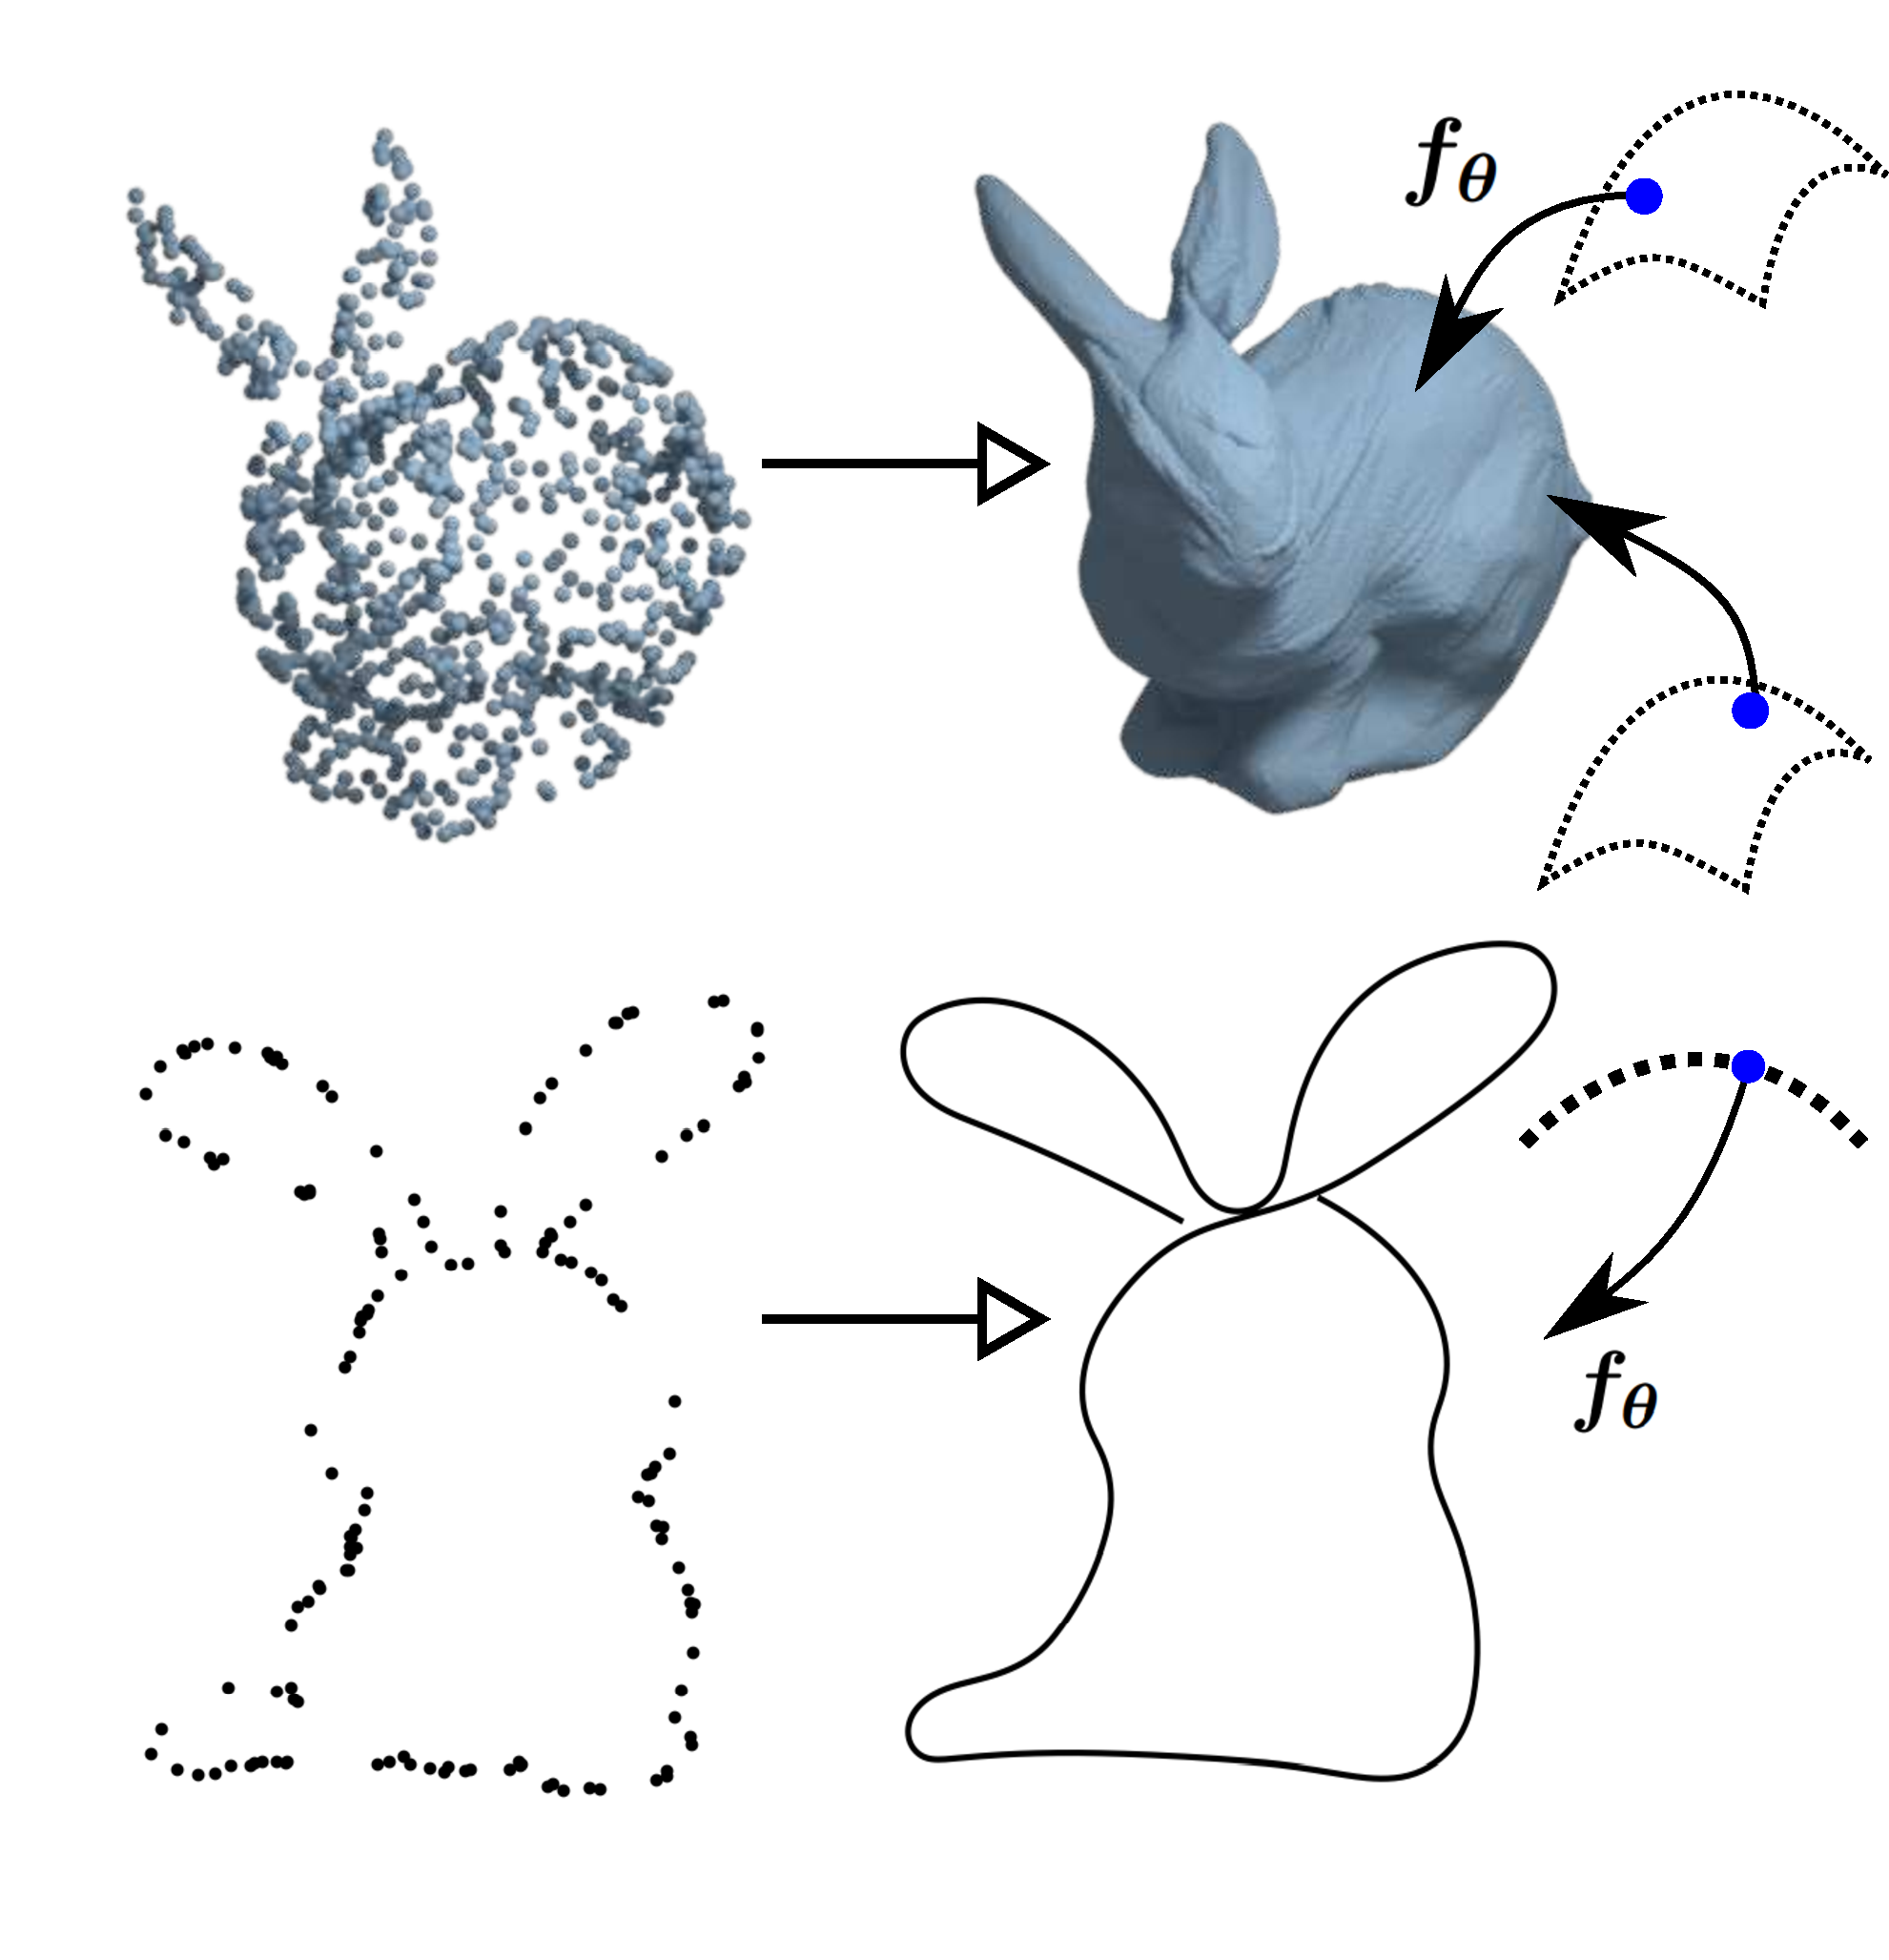
\includegraphics[width=0.5\linewidth]{dmp/imgs/visabstract.pdf}
\caption{\label{fig:visabstract}\small
\textbf{Deep manifold prior}. Points interpolated by using deep networks to map points in a 2D grid~(top) and 1D grid~(bottom) to the target shape (a 3D surface and a 2D curve respectively). The networks are randomly initialized and trained to minimize the Chamfer distance to the target.}
\end{figure}

\section{Introduction}

In recent years a variety of approaches have been proposed to generate manifold data such
as surfaces of 3D shapes using deep networks.
The goal of this work is to characterize how the choice of the network architecture
impacts the properties of the resulting surfaces.
We present and analyze a \emph{deep manifold prior}, an approach to represent a
manifold as a collection of transformations (atlas) of an
Euclidean space parameterized using deep networks (Section~\ref{dmp:method}).
We show that random networks induce smooth surfaces whose limiting
behavior can be understood in terms of a Gaussian process
(GP)~\cite{Neal,williams1997computing, cho2009kernel}.
We analyze how the different network architectures affect the
distribution of position, normals and
curvature of surfaces (Section~\ref{sec:gp}).
We also derive the properties of implicit surfaces 
induced by the level-set of a scalar field \{$f(x) = c$\} parameterized
using a deep network.


\begin{figure*}[ht]
\centering
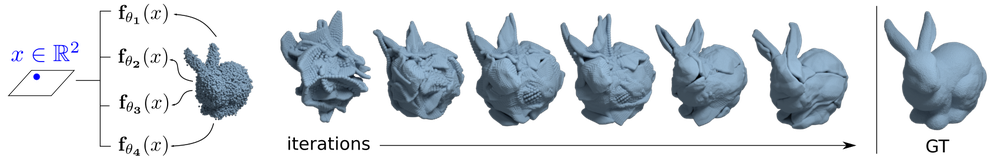
\includegraphics[width=\linewidth]{dmp/imgs/iters.png}
    \caption{\label{fig:pipeline} \small \textbf{Manifold reconstruction pipeline.}
    Manifold parametrizations are encoded by neural networks ($\mathbf{f_{\theta_i}}$)
    and trained to minimize the reconstruction error with respect to the noisy target
    (left).
    Prior induced by the neural networks makes the generated surface much closer to
    the ground-truth (right), without ever seeing any additional training data.
}
\end{figure*}

As a concrete application we study the problem of 
interpolating and denoising point clouds sampled from contours or surfaces of
shapes, as seen in Figures~\ref{fig:visabstract} and~\ref{fig:pipeline}.
The manifold parametrization allows us to efficiently sample point
clouds, which can be combined with a Chamfer metric to measure a
reconstruction error with respect to the sampled data. 
We show that smooth surfaces are obtained when the parameters of the networks are learned to minimize the reconstruction error starting from a \emph{random initialization} (Figure~\ref{fig:pipeline}).
The approach is also effective for the level-set formulation, where the objective is to learn a deep network that correctly classifies points as \emph{inside} or \emph{outside} the surface.
However, an advantage of the explicit parametrization is that it does
not require the notion of what is inside.
In addition we introduce a \emph{regularization} that reduces self-intersections, overlaps, and distortion of the parametrization, which is desirable for applications such as texture mapping ~(Section~\ref{dmp:method}).
Our approach requires \emph{no} prior learning, works across a range of 3D
shapes, and outperforms strong baselines for point cloud denoising, 
such as Screened Poisson Surface Reconstruction (SPSR) and Robust Implicit Moving Least Squares (RIMLS).
It is also more lightweight than approaches that
operate on volumetric representations of 3D shapes (Section~\ref{dmp:experiments}).

Our analysis sheds lights on the impressive performance of several
recently proposed architectures for 3D surface generation, such as
MRTNet~\cite{mrt18}, AtlasNet~\cite{atlasnet}, FoldingNet~\cite{yang2018foldingnet}, and Pixel2Mesh~\cite{pixel2mesh}, as well as implicit surface approaches~\cite{chen2019learning,mescheder2019occupancy,genova2019learning,park2019deepsdf}.
These can be be interpreted
as different ways of parameterizing a manifold.
In particular, AtlasNet generates a 3D shape as a collection of surfaces, each represented as a
transformation of a unit grid using a fully-connected network.
However, the generated pieces exhibit significant overlap which
results in a poor surface reconstruction and is less desirable for
applying materials and textures to the surface (Section~\ref{dmp:experiments}).
The proposed regularization alleviates this problem. 
Moreover, by replacing the fully-connected networks of AtlasNet with
convolutional variants we improve the performance on standard
benchmarks for shape generation~\cite{choy20163d} with networks that have a
fraction of the parameters, faster inference time, as well
as smaller memory footprint (Section~\ref{dmp:experiments}).
